\documentclass[tikz,border=5pt]{standalone}
\usetikzlibrary{arrows.meta,positioning}
\begin{document}
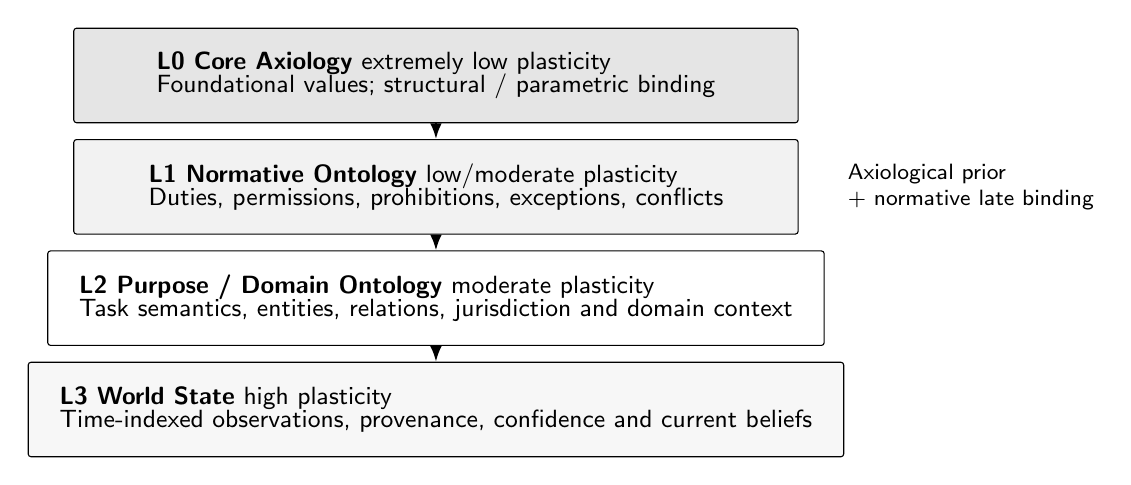
\begin{tikzpicture}[
  layer/.style={draw, rounded corners=1pt, minimum width=92mm, minimum height=12mm, align=left, font=\sffamily\small, inner xsep=4mm},
  arrow/.style={-{Latex[length=2mm]}, thick}
]
\node[layer, fill=black!10] (l0) {\textbf{L0 Core Axiology} \hfill extremely low plasticity\\[-1mm] Foundational values; structural / parametric binding};
\node[layer, fill=black!5, below=2mm of l0] (l1) {\textbf{L1 Normative Ontology} \hfill low/moderate plasticity\\[-1mm] Duties, permissions, prohibitions, exceptions, conflicts};
\node[layer, fill=white, below=2mm of l1] (l2) {\textbf{L2 Purpose / Domain Ontology} \hfill moderate plasticity\\[-1mm] Task semantics, entities, relations, jurisdiction and domain context};
\node[layer, fill=black!3, below=2mm of l2] (l3) {\textbf{L3 World State} \hfill high plasticity\\[-1mm] Time-indexed observations, provenance, confidence and current beliefs};
\draw[arrow] (l0) -- (l1);
\draw[arrow] (l1) -- (l2);
\draw[arrow] (l2) -- (l3);
\node[font=\sffamily\footnotesize, right=5mm of l1, align=left] {Axiological prior\\+ normative late binding};
\end{tikzpicture}
\end{document}
